\documentclass[paper=a4, fontsize=11pt]{scrartcl} %twocolumn, 

\usepackage[utf8]{inputenc} % Use 8-bit encoding that has 256 glyphs

%\usepackage{fourier} % Use the Adobe Utopia font for the document - comment this line to return to the LaTeX default
\usepackage[english]{babel} % English language/hyphenation
\usepackage{amsmath,amsfonts,amsthm, amssymb} % Math packages, use \sim to get tilde

\usepackage{graphicx} % Required for including pictures

\usepackage{booktabs} % Allows the use of \toprule, \midrule and \bottomrule in tables for horizontal lines

%----------Pasting Code---------------

\usepackage{listings} % \usepackage{listings} For inserting code into the document
% Using \usepackage{listingsutf8} for multi-byte encoding of source code

\lstset{breaklines = true, 
numbers = left, 
commentstyle = \color{mygreen}, 
keywordstyle = \color{blue}, 
stringstyle = \color{mymauve},
showstringspaces = true
}
%inputencoding = utf8, 
%extendchars = \false

%\usepackage{minted}
\usepackage{color} %for syntax highlighting

\definecolor{mygreen}{rgb}{0,0.6,0}
\definecolor{mygray}{rgb}{0.5,0.5,0.5}
\definecolor{mymauve}{rgb}{0.58,0,0.82}

%------------END--------------

\usepackage{float} %for aligning figures

\usepackage{wrapfig} %for using wraptable or wrapfig

\usepackage{caption}
\usepackage[l2tabu]{nag}

%\usepackage[nottoc]{tocbibind} %to include the bibliography in the contents

\usepackage{verbatim} %use \begin{comment} and \end{comment}. For more complex tasks, check out package:comment

\usepackage{bm} % for printing greek symbols in bold, use \boldsymbol\varepsilon

\usepackage{rotating} % for rotating tables
\usepackage{longtable} % for long tables, 

\usepackage{subcaption} %for supressing table numbering in subtables
\usepackage{makecell} %for multiple lines in a table, enclose the cell value in \thead{A \\ B}

\usepackage{lscape} %for rotating the page with the long table

\usepackage{todonotes} %add TODOs by putting the text in \todo{}

\usepackage{csquotes} %use \begin{displayquotes} to enter a quote

% for changing the nature of urls
%\usepackage[hidelinks]{hyperref} %hides hyperlinks
\usepackage[linktoc = none, linkbordercolor	={0 1 0}]{hyperref}

% custom commands
\newcommand{\mytilde}{\raise.17ex\hbox{$\scriptstyle\mathtt{\sim}$}}

\usepackage{fancyhdr} % Custom headers and footers
\pagestyle{fancyplain} % Makes all pages in the document conform to the custom headers and footers
%\fancyhead{} % No page header - if you want one, create it in the same way as the footers below
\fancyhead[L]{}
\fancyfoot[L]{} % Empty left footer
\fancyfoot[C]{\thepage} % Page numbering for right footer
\fancyfoot[R]{} % Empty right footer
\renewcommand{\headrulewidth}{0pt} % Remove header underlines
\renewcommand{\footrulewidth}{0pt} % Remove footer underlines
\setlength{\headheight}{13.6pt} % Customize the height of the header

\numberwithin{equation}{section} % Number equations within sections (i.e. 1.1, 1.2, 2.1, 2.2 instead of 1, 2, 3, 4)
%\numberwithin{figure}{section} % Number figures within sections (i.e. 1.1, 1.2, 2.1, 2.2 instead of 1, 2, 3, 4)
%\numberwithin{table}{section} % Number tables within sections (i.e. 1.1, 1.2, 2.1, 2.2 instead of 1, 2, 3, 4)

\setlength\parindent{5pt} % Removes all indentation from paragraphs - comment this line for an assignment with lots of text

\graphicspath{{/home/ad/Desktop/images/}} % Specifies the directory where pictures are stored

%----------------------------------------------------------------------------------------
%	Some Tips For Using This Template
%----------------------------------------------------------------------------------------


\begin{comment}

\end{comment}

%----------------------------------------------------------------------------------------
%	TITLE SECTION
%----------------------------------------------------------------------------------------

\rhead{Akshat Dwivedi}
\lhead{Data Mining \& Neural Networks}
%\rfoot{\begin{picture}(0,0) \put(-45,-100){\includegraphics[width=3cm]{KU_LeuvenFR}} \end{picture}}
\newcommand{\horrule}[1]{\rule{\linewidth}{#1}} % Create horizontal rule command with 1 argument of height

\title{	
\normalfont \normalsize 
\textsc{\Large KU Leuven} \\ [30pt] % Your university, school and/or department name(s)
\horrule{0.5pt} \\[0.4cm] % Thin top horizontal rule
\huge Data Mining and Neural Networks: \textbf{Update} \\ % The assignment title
\horrule{2pt} \\[0.5cm] % Thick bottom horizontal rule
}

\author{Akshat Dwivedi (Student Number: blah blah)\\
\\
Instructor: Prof. Johann Suykens\\
Course: G9X29A} % Your name

\date{January 22, 2015} % Today's date or a custom date

\pagenumbering{arabic}

%--------------------------------------------------------------------------------

\begin{document}

\maketitle % Print the title

\tableofcontents

%\thispagestyle{empty}
\clearpage
\setcounter{page}{1}

%\listoftodos %makes a list at the top of the document with TODOs

% Begin writing here:
\section{Curse of Dimensionality}
\subsection{m = 2}
Similar to the case for m=1, the aim is to use a neural network to train the \texttt{sinc} function for 2 dimensions. This function is also known as the mexican hat function. A plot of this function over the 2-dimensional interval $[-5,5]^2$ is given in figure \ref{sinc2}.

\begin{figure}[h]
\centering
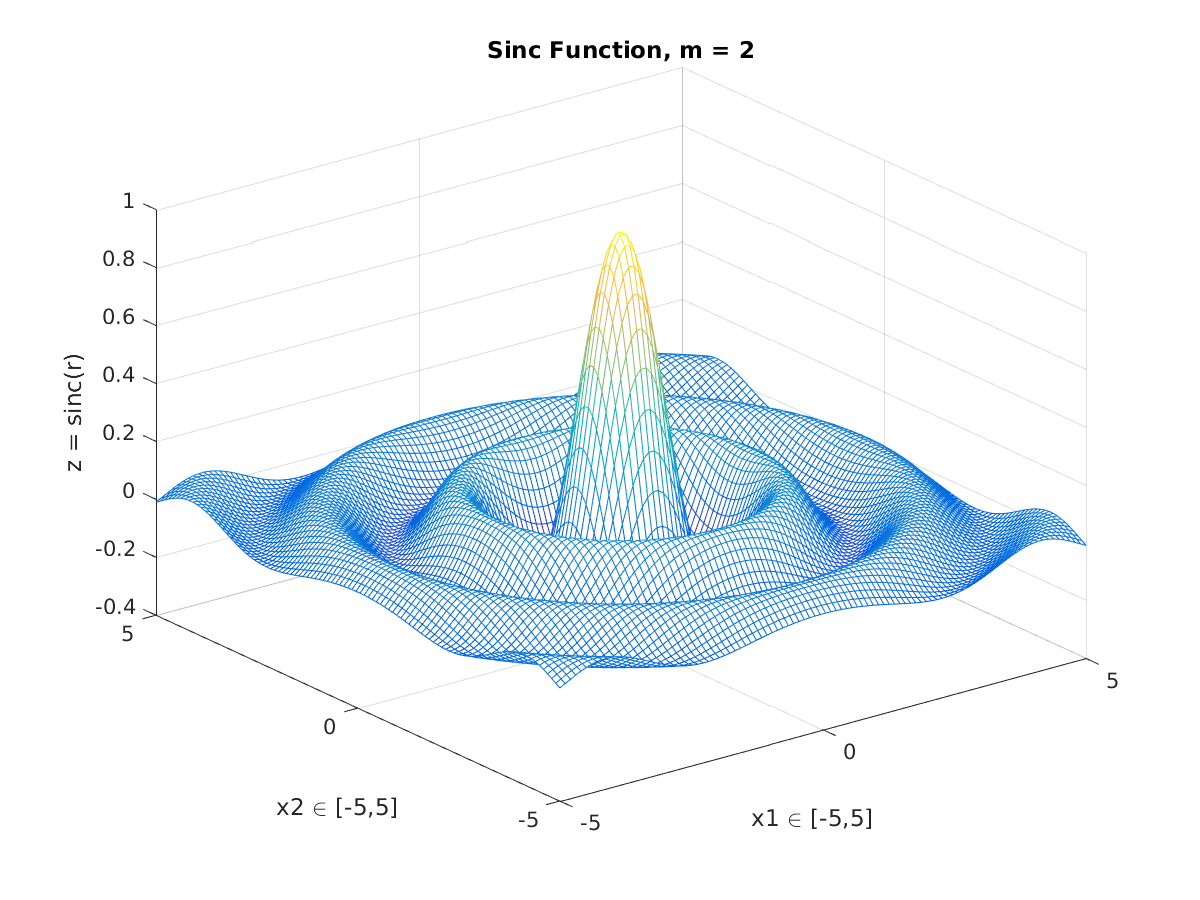
\includegraphics[width = 0.8\textwidth]{sinc2.png}
\caption{Mexican hat function on the 2-dimensional interval $[-5,5]^2$}
\label{sinc2}
\end{figure}

It is interesting to note, that in the 1-dimensional case, 100 points were used (training set) and there was a lesser amount of "empty space" in the plot. Comparing this to the 2-dimensional case, we see that there is a lot more "empty space" in 3-dimensions compared to 2-dimensions. If we take 100 equally spaced points for $x_1$ and $x_2$ $\in [-5,5]$, we get a grid of $100^2$ = 10,000 points in the training set. Thus, we observe that the number of cases $n$ has now increased from 100 to 10,000. Generally speaking, for an $m$-dimensional input space, the training set would contain 10$^m$ cases. This is known as the \emph{curse of dimensionality}.\\

We decide to go with the full training set with 10,000 points and use early stopping with a validation set consisting of 53 equally spaced points on [-4.9,4.9]. Thus, the validation set consists of 53$^2$ = 2809 points. Finally, a separate test set of 40$^2$=1600 points on [-4.8,4.8]$^2$ is created to evaluate the network performance and is not used at the time of training the network. The advantage of selecting these three sets is that they are mutually disjoint and hence, the network is evaluated on sets which are similar, but not the same as the training set. The activation function function used is the radial basis function which is selected due to it's advantage in using a smaller number of neurons. Levenberg-Marquadt algorithm is used to train the network due to it's fast convergence rate, however resilient backpropagation was tried and resulted in a poorer fit compared to the LM algorithm. The network was trained with 25 and 35 neurons. 

\begin{figure}[h]
	\begin{subfigure}{0.5\linewidth}
		\centering
		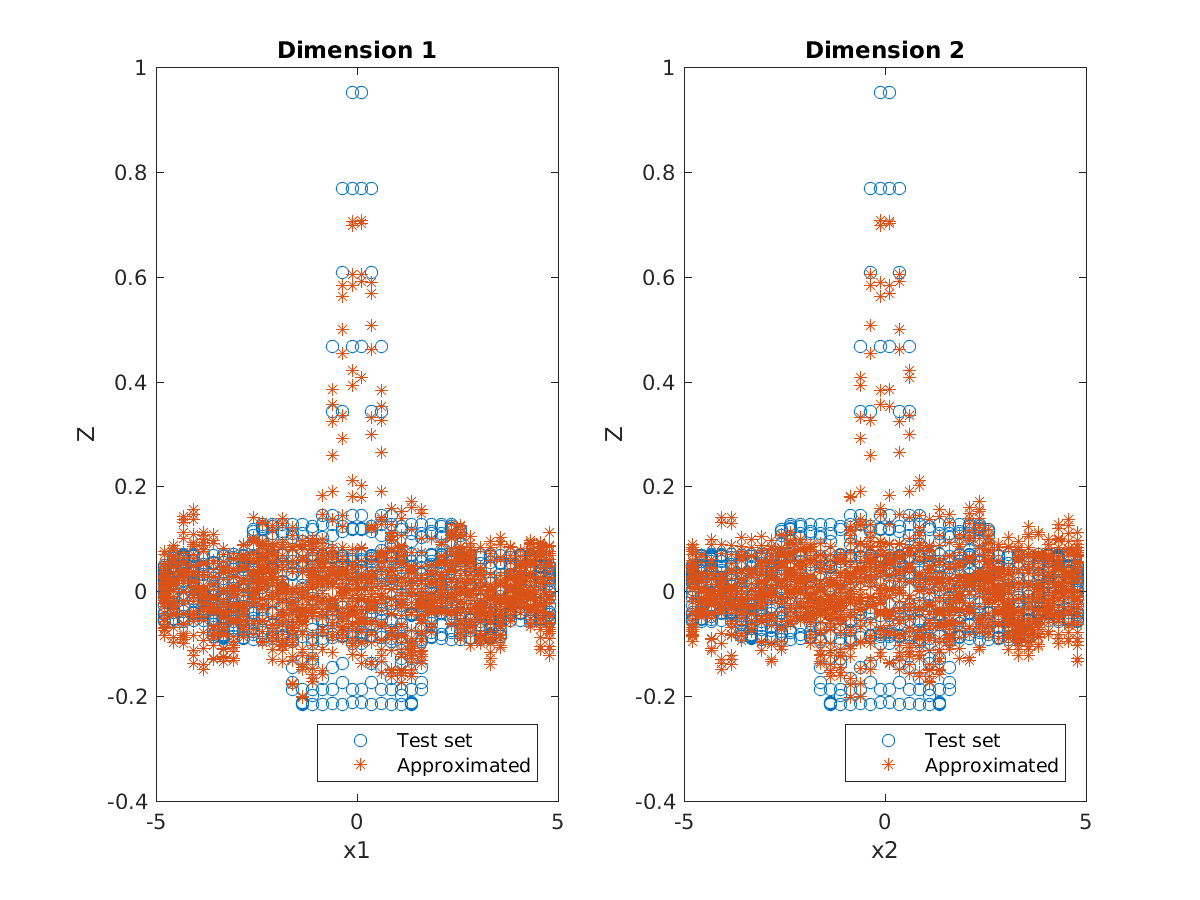
\includegraphics[width = \textwidth]{sinc2point25.png}
		\caption{25 neurons}
	\end{subfigure}
	\begin{subfigure}{0.5\linewidth}
		\centering
		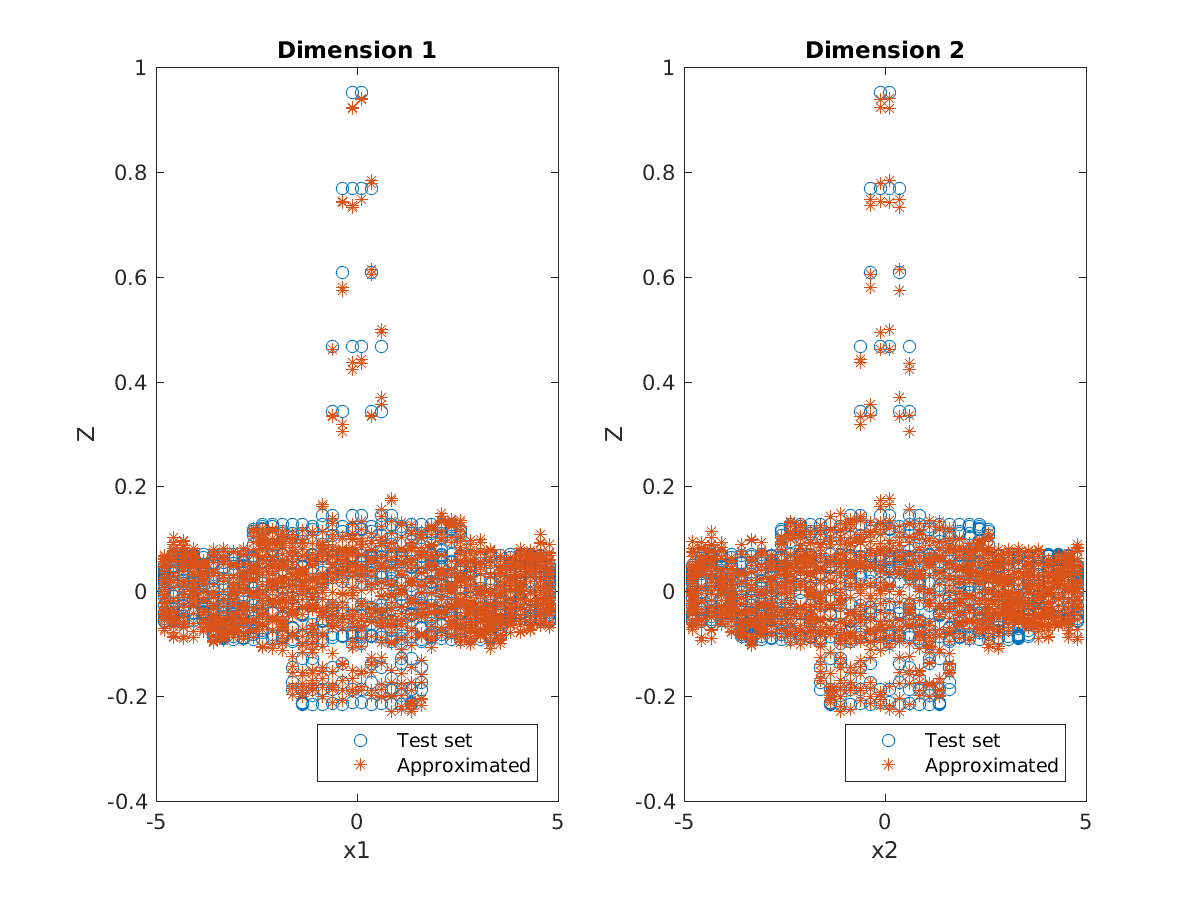
\includegraphics[width = \textwidth]{sinc2point35.png}
		\caption{35 neurons}
	\end{subfigure}
\caption{Mexican hat function in 2 dimensions. Plot of the test set with the approximated function on the test set. 25 and 35 neurons were tried.}
\label{sinc2fit}
\end{figure}

In figure \ref{sinc2fit}(a), we see that the network with 25 neurons is not able to adequately approximate the underlying function. The MSE on the test set  is 0.0039. In \ref{sinc2fit}(b) we see that the performance of the network with 35 neurons results in a rather good fit. The MSE was found to be 0.000494.

\subsection{m = 5}
Now we arrive at the interesting part of the exercise: evaluating the \texttt{sinc} function in 5 dimensions. The first problem we run into is that the training and test sets cannot be chosen in a manner that was employed for the 1- and 2-dimensional cases. Selecting 100 equally points on a 5-dimensional grid, for example, will lead to $100^5$=10,000,000,000 observations which is simply too impractical. Furthermore, it would be challenging to visualize the approximated function due to the dimension being greater than 3.\\ 

Thus, we compare the fitted models based on MSE on the training and test sets. 5 networks are trained with 100, 200, 300, 400 and 500 nodes in the hidden layer. Furthermore, we used the scaled conjugate gradient algorithm to train the network as it is suitable for large scale problems as it does not store large matrices in memory. Training set was chosen to be 15 equally spaced points on the $[-5,5]^5$ interval which results in $15^5$ = 759375 cases used to train the network. A validation set of 10 equally spaced points was chosen on the $[-4.9,4.9]^5$ which resulted in 100000 cases in the validation set. Similarly, a test set of 10 equally spaced points was chosen on the $[-4.8,4.8]^5$ which resulted in 100000 cases in the test set. Early stopping was used to train the network, however, due to time constraints, we trained the network for 200 epochs and training was stopped whichever of these two occurred first. It was observed that increasing the number of neurons did not improve the fit. An attempt was made to assess convergence with the Levenberg-Marquadt algorithm, however, the training time was simply too high.\\

This indicates that the successes of this approach for the 1- and 2-dimensional cases would not be appropriate here. Thus, we would have to resort to sampling methods to choose the training set on $[-5,5]^5$. Uniformly sampling from this interval will not result in adequate  training sets, as it will be give higher weight to the observations away from the center than the case for the sinc function. Sampling from a weighted mixture distribution might result in an adequate training set. This appears to be a non-trivial task.

\begin{comment}
\begin{table}
\centering
\begin{tabular}{|c|c|c|}
\hline
Hidden units & Training Set & Test sets \\ 
\hline
100 & 	0.0014	& 0.0014 \\
\hline
200 & 	& \\
\hline
300 & 	& 	\\
\hline
400 & 	& \\
\hline
500	& 	& \\
\hline
\end{tabular}
\caption{MSE of the network on the test set for the sinc function in 5 dimensions.}
\label{sinc5}
\end{table}
\end{comment}

\begin{comment}
\section{Appendix (MATLAB Code)}
\subsection*{Session 1}
\lstinputlisting[language = Matlab, frame = single, firstline = 170]{"/home/ad/Desktop/KUL Course Material/Data Mining And Neural Networks/Final exam/exercise1.m"}
\end{comment}

%---------------------------------------------
\end{document}